\chapter{Тройное сальто назад можешь? Трюки и фишечки}
\label{ch:tricks}

Далее пойдет речь о красивых приемах игры, которые лучше осваивать не с листа бумаги, а под присмотром и руководством опытного гитариста. Ощутимо могут помочь видеоролики, поэтому не поленитесь и зайдите, например, на Youtube-канал\footnote{От себя: очень рекомендую Youtube-канал <<Гитара с нуля --- уроки игры на гитаре>> \cite{url:guitarFromZero}, как полноценный обучающий курс, построенный по принципу от простого к сложному. Канал <<Нескучный саунд>> \cite{url:funnySound} хорош для тех, кто подкован в музыке стальными подковами. Электрогитаистам стоит обратить внимание на канал <<fredguitarist>> \cite{url:fredguitarist}, предварительно отсеяв замечательные уроки от отвратительных поливаний грязью всех остальных гитаристов} <<Pima Live>> \cite{url:pimalive}.


\section{А чтоб как капелька упала? Флажолет}
\label{ch:tricks:flageolet}

Флажолетом называется прием игры, позволяющий <<изъять>> из обычного звука оснвоной тон и часть обертонов. В результате получается весьма необычный на слух звук.

Для начала вспомним структуру звука, издаваемого струной, обратившись к рисунку \ref{fig:tricks:flageolet:nodes}. Заметим, что в помеченных на рисунке серыми кружками точках струны колебания отсутствуют --- это узлы колебаний. Первый обертон имеет один узел на струне, второй --- два, и тд.

\begin{figure}[!ht]
    \centering
    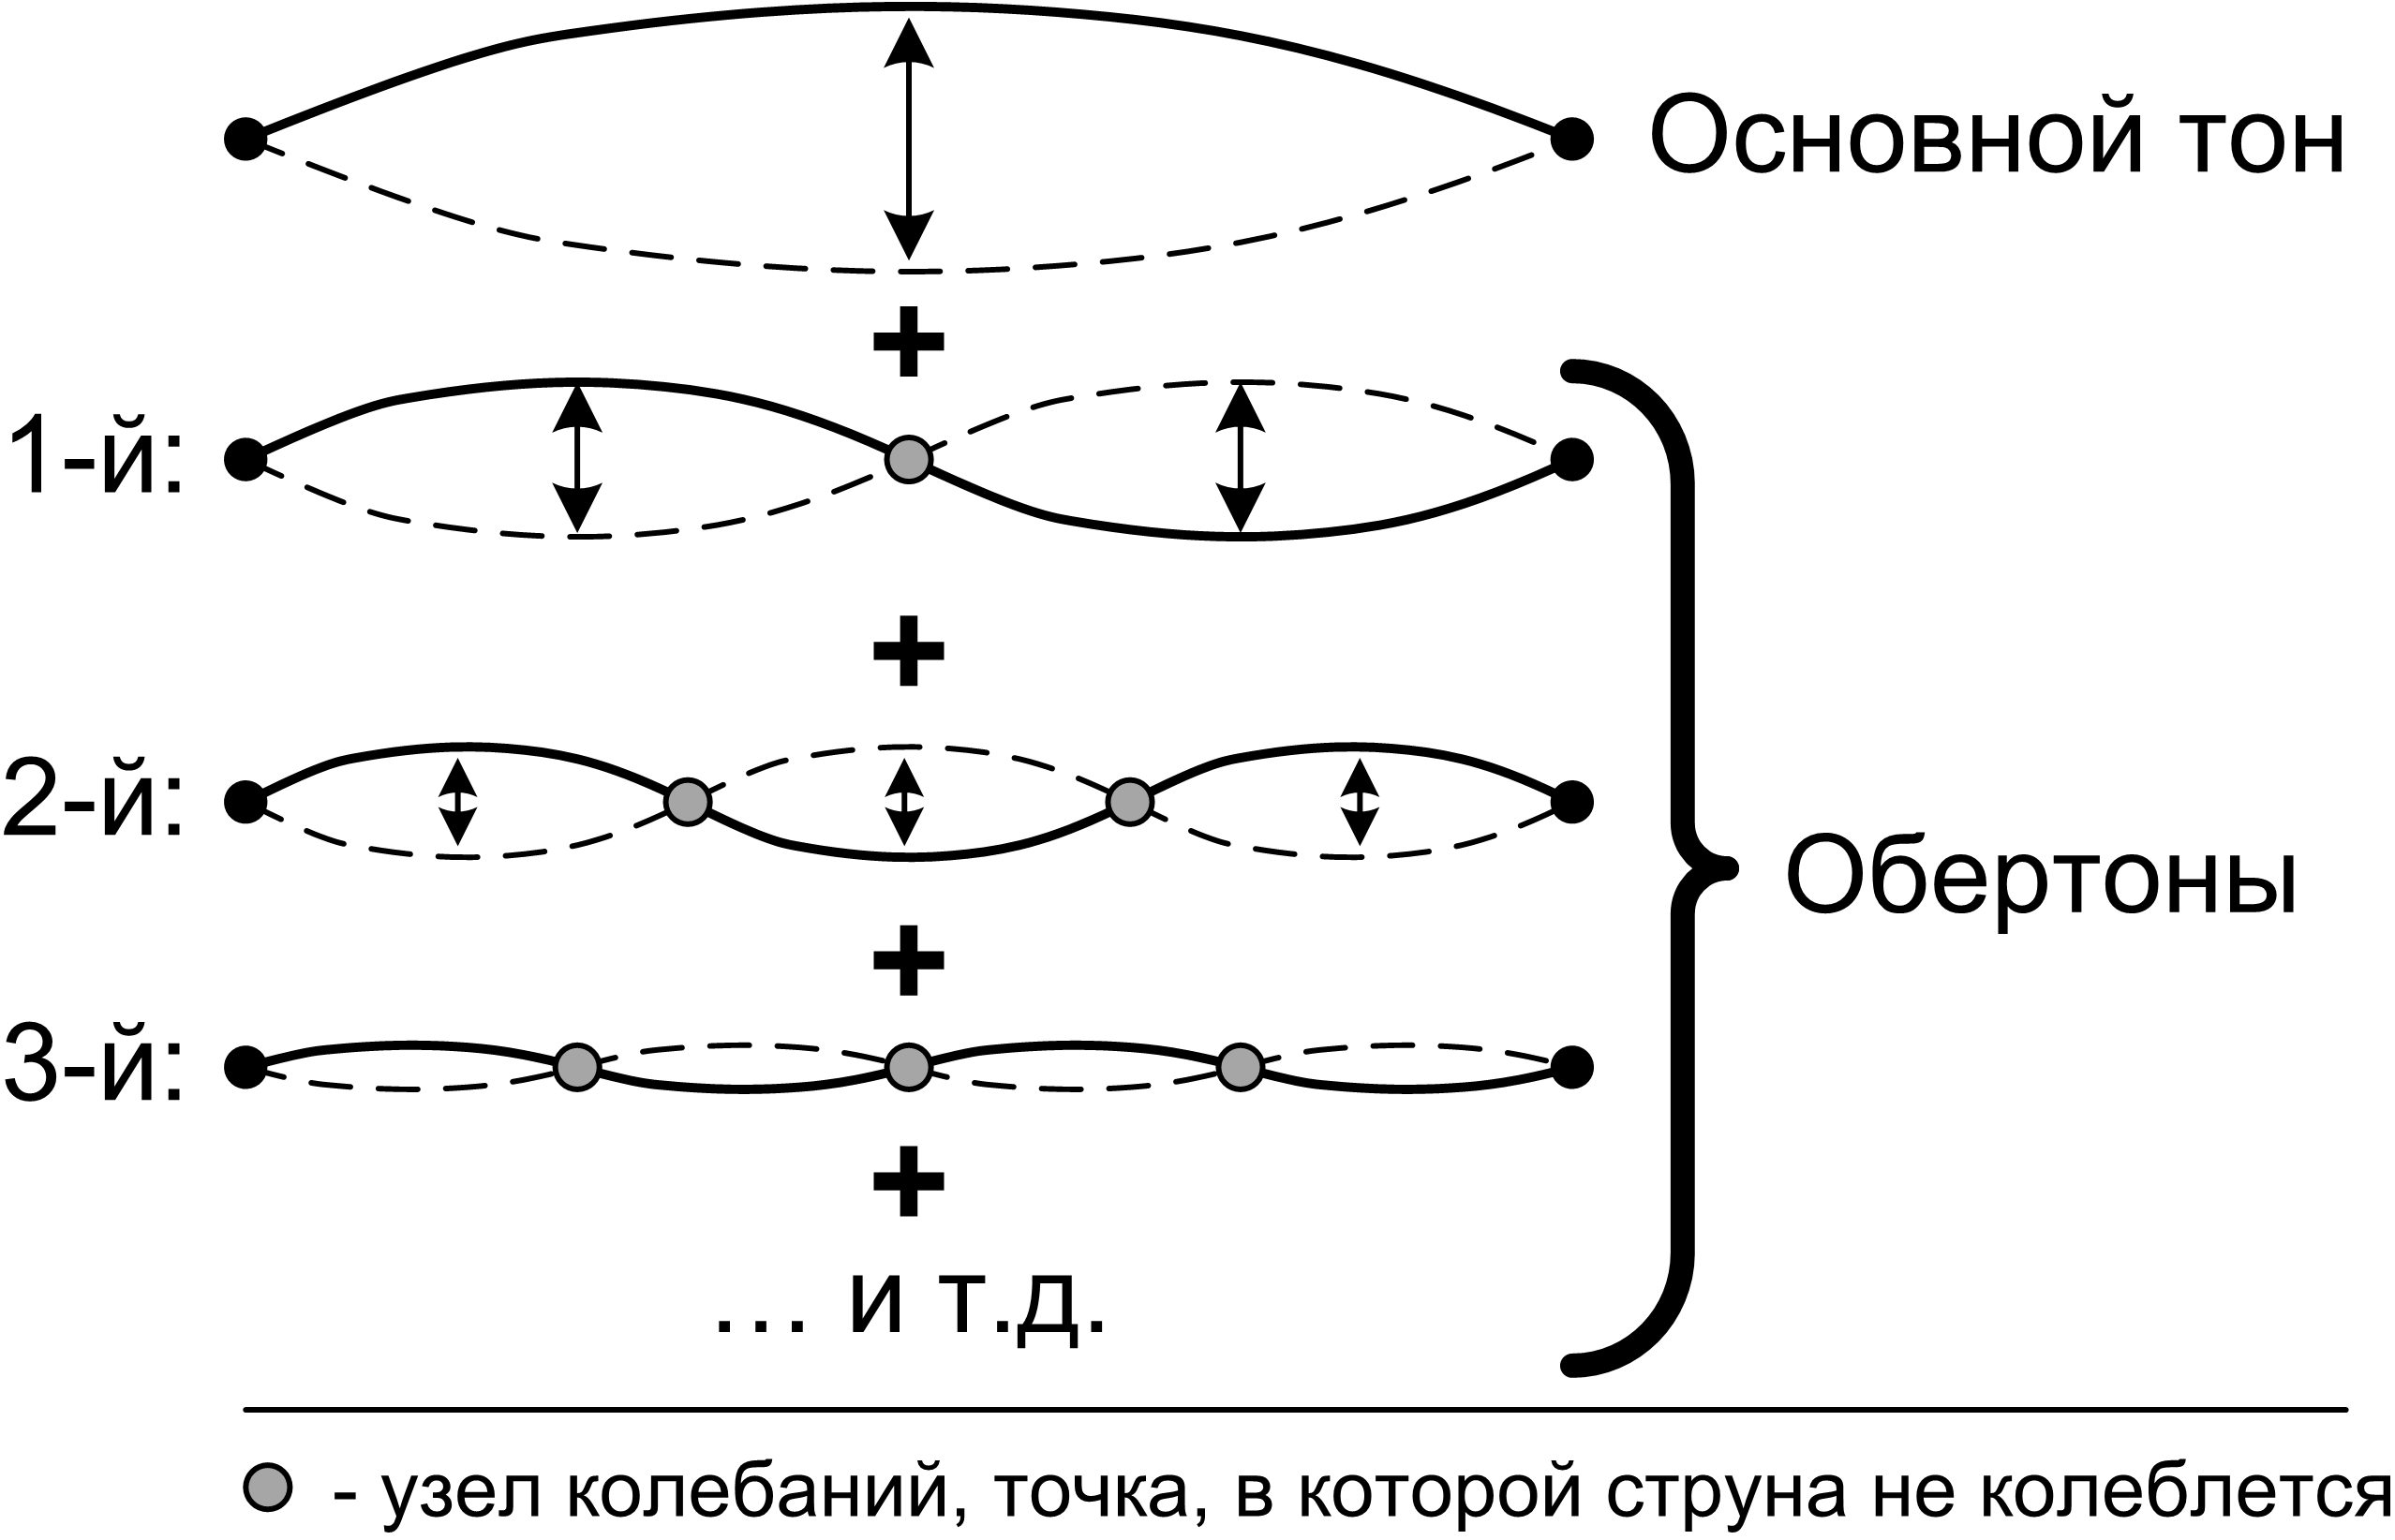
\includegraphics{fig/string-nodes} 
    \caption{Структура звука}\label{fig:tricks:flageolet:nodes}
\end{figure}

\begin{Example}[Сыграем первый флажолет]
    Давайте сыграем флажолет на первой, самой тонкой струне. Там он прозвучит лучше всего. Найдем середину струны --- место, где находится узел первого обертона. Как известно, это прямо над 12-м ладовым порожком. Далее нужно легко поставить палец\footnote{Обычно указательный или средний, какой лучше слушается} левой руки на середину струны, не нужно сильно давить, а тем более прижимать струну к 12-му порожку --- нужно легкое касание. Далее щипните правой рукой струну как обычно, но чуть порезче. Палец левой руки должен уйти с узла вверх на мгновение позже щипка, почти одновременно с ним.
    
    Попробуйте несколько раз, вы поймете, когда у вас получится. Поищите нужное движение, при котором звук получается наиболее ярким.
    
    Причина постоянных неудач: палец левой руки стоит не на узле. 
    
    Если всё получилось, попробуйте сыграть флажолет над 11 или 13-м ладами. Не получается? И не должно. Флажолет - капризная штука, не правда ли?
    
    Что получилось в результате такого приема извлечения звука? Палец левой руки заглушил основной тон, а также все обертоны, не имеющие узла в середине струны. Громче всех (вместо основного тона) прозвучит при этом 1-й обертон.
    
    Разница между сыгранным нами флажолетом и обычным щипком на 12 ладу изображена на рисунке \ref{fig:tricks:flageolet:first}.
\end{Example}
 
\begin{figure}[!ht]
    \centering
    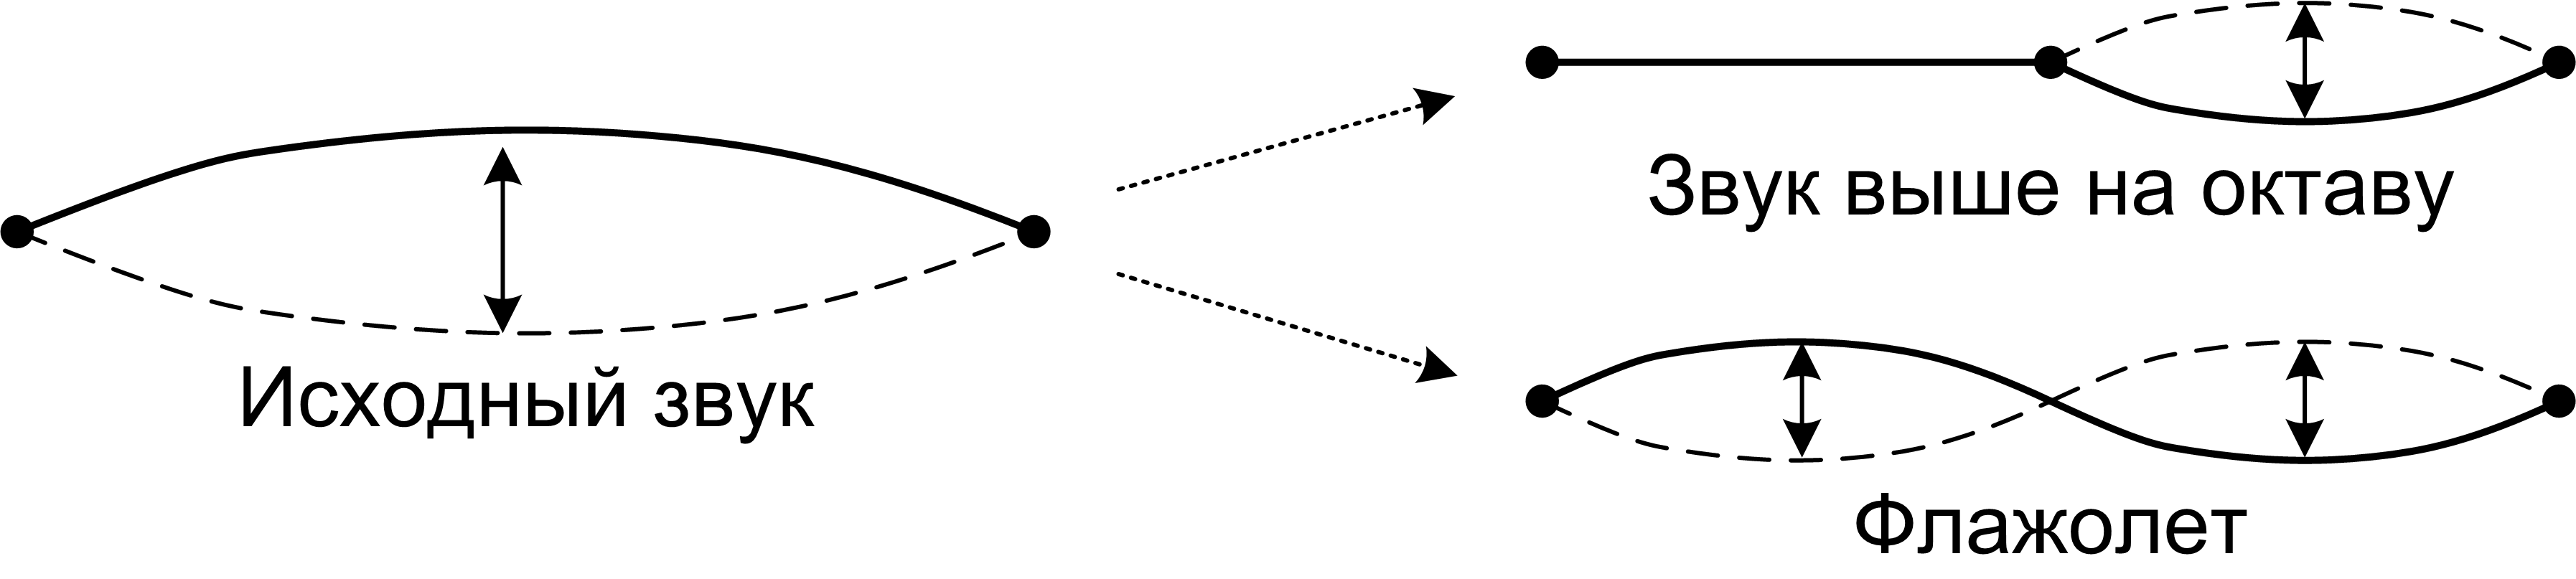
\includegraphics{fig/string-flageolet} 
    \caption{Флажолет первого порядка}\label{fig:tricks:flageolet:first}
\end{figure} 

Этим же приёмом можно сыграть флажолет в узле, делящем струну на три части (см. второй обертон на рисунке \ref{fig:tricks:flageolet:nodes}). В этом случае один из узлов будет находится примерно на 7-м ладу. Давайте проверим, опираясь на формулу \ref{fig:guitar:construction:length} (и помня, что это формула длины струны от подставки до лада):
\[
    L(7)=\frac{L}{(\sqrt[12]{2})^7}\approx L\cdot 0.66742
\]

Тогда как необходимые нам $\frac{2}{3}\cdot L$ составляют:
\[
    \frac{2}{3}\cdot L \approx L\cdot 0.66667
\]

Абсолютная погрешность будет равна $\Delta \approx 0,00075 \cdot L$. Так как длина струны $L$ на полноразмерной классической гитаре составляет $66$ см., то погрешность составит меньше половины миллиметра. Поглядите на свой пухленький пальчик и смело пренебрегайте погрешностью --- ставьте палец левой руки прямо над 7-м ладом.

Играя флажолет на трети струны, вы столкнетесь с еще одним фактором, влияющим на качество звука: флажолет не прозвучит, если правая рука будет щипать струну вблизи второго узла (треть струны от подставки). Поэкспериментируйте. Капризов у флажолета добавилось.

Четверть струны находится примерно над 5-м ладовым порожком\footnote{Буквоеды, посчитайте погрешность}. Не забывайте о наличии уже трех узлов колебаний, вблизи которых нельзя щипать струну правой рукой.

На этом пожалуй можно остановиться, потому что флажолеты более высоких порядков играть все сложнее: они звучат все тише и тише, а вероятность ошибки все больше и больше.

Мы разобрали флажолеты на открытых струнах. Музыканты называют их натуральными или естественными. Так как на практике играют флажолеты в основном на половине струны, и гораздо реже на трети или четверти, то вариантов не слишком-то много.

Представим, что вы зажали струну на первом ладу и она стала короче. На каком ладу теперь находится половина струны? Правильно, на 13-м! Сомневаетесь --- поковыряйте формулу \ref{fig:guitar:construction:length}. На каком бы ладу вы не зажали струну, её половина будет находится на 12 ладов выше, треть --- на 7, четверть --- на 5. Количество мест, где можно сыграть флажолет, резко возросло.

И это, конечно здорово, но если мы зажимаем лад левой рукой, то где взять еще одну руку, чтобы придерживать узел? На открытой струне это делалось левой рукой. Увы, если у вас нет лишней руки, то справляться придется одной правой. Обычно правая рука делает это так: указательным пальцем касается нужного узла, а большим (безымянным или мизинцем, кому как удобнее) играет щипок, практически одновременно с этим снимая с узла указательный палец (проще отнимать ладонь целиком). Знакомьтесь: \emph{искуственный} флажолет.

Все, что сказано, справедливо для аккустических гитар\footnote{В отношении колебаний струны справедливо, конечно и для электрических гитар тоже. Но флажолеты на электрических гитарах играют по-другому. Если задеть колеблющуюся струну на аккустике, то звук исчезнет почти сразу --- слишком много энергии потеряет струна. Но это не значит, что она перестанет колебаться. Таким касанием отфильтруется основной тон и огромное количество обертонов. Останутся только обертоны с узлами в точке касания. Так как электрическая гитара сосет энергию для звука из электрической сети, то её потери энергии струны волнуют гораздо меньше --- больше важен сам факт колебаний. То есть на электрогитаре долго мучаться с поиском нужного узла не надо вовсе --- ткните в любое место на струне и результат будет. Сам флажолет на электрогитаре звучит не так изящно, как на аккустике --- он визжит (словами А. Пушного) <<как сучка>>! Обычно флажолет на электрогитаре играют так: медиатор резко ударяет по струне, его движение продолжается чуть дальше, чем обычно, а один из пальцев правой руки на мгновение касается струны}.


\section{А нужен молоток? Hammer-on, hammer-off}

\section{Как выжать слезу? Вибрато}
\label{ch:tricks:vibrato}

Когда звук сыгран правой рукой, а палец левой руки, прижимающий струну примерно посередине между ладовыми порожками, за счет движения запястья и предплечья как бы <<прокатывается>> подушечкой туда-обратно вдоль струны, возникает очень выразительный, рвущий душу на части звук.  

\begin{figure}[!ht]
    \centering
    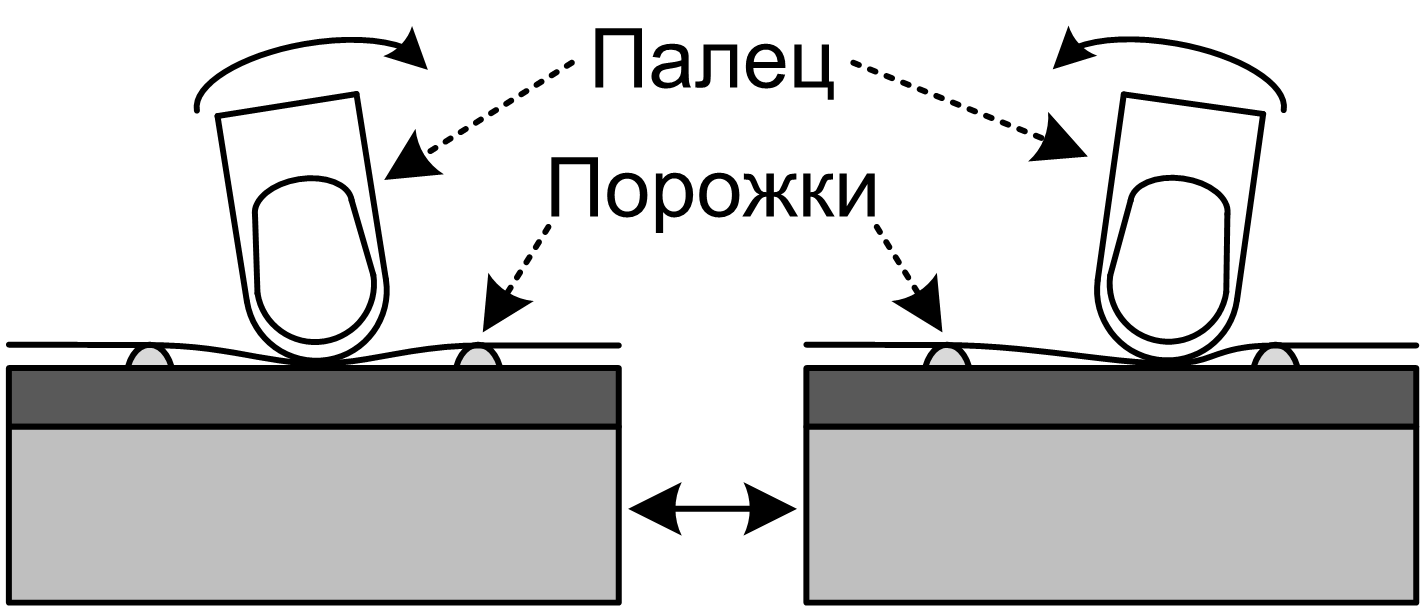
\includegraphics{fig/vibrato} 
    \caption{Структура звука}\label{fig:tricks:vibrato}
\end{figure}

Едва уловимые периодические биения высоты основного тона привлекают к себе внимание. Это происходит из-за незначительных изменений натяжения струны, когда по ней прокатывается подушечка пальца. На рисунке \ref{fig:tricks:vibrato} видно, что участок струны между ладами в разных положениях имеет разную длину, а значит из-за этого изменилось и натяжение струны в целом.


\section{Подтяжки? Подтяжка}


